\documentclass{beamer}
\usepackage[utf8]{inputenc}
\usepackage[T1]{fontenc}
\usepackage{lipsum, lmodern}

% za figure
\usepackage{wrapfig}
\usepackage{hyperref}
\usepackage{amsmath}
\usepackage{graphicx}
\usepackage{subfig}

% farebne tabulky
\usepackage {colortbl}

\newcommand {\tab} {\indent}

%\usetheme{Median}
\usetheme{CambridgeUS}

% Cesta k obrazkam
\graphicspath{ {pics/} }

%pre figure
\usepackage{alphalph}
\renewcommand*{\thesubfigure}{%
\alphalph{\value{subfigure}}%
}%

\setbeamertemplate{footline}{%
    \leavevmode%
    \hbox{
        \begin{beamercolorbox}[wd=.2\paperwidth,ht=2.5ex,dp=1.125ex,leftskip=.2cm, rightskip=.3cm]{author in head/foot}%
            \usebeamerfont{author in head/foot}\insertshortauthor
        \end{beamercolorbox}%
        \begin{beamercolorbox}[wd=.55\paperwidth,ht=2.5ex,dp=1.125ex,leftskip=.2cm,rightskip=.3cm plus1fil]{title in head/foot}%
            \usebeamerfont{title in head/foot}\insertshorttitle
        \end{beamercolorbox}%
        \begin{beamercolorbox}[wd=.25\paperwidth,ht=2.5ex,dp=1.125ex,leftskip=.2cm,rightskip=.3cm plus1fil]{date in head/foot}%
            \usebeamerfont{date in head/foot}\insertshortdate\qquad \insertframenumber/\inserttotalframenumber
        \end{beamercolorbox}}%
    \vskip0pt%
}

\author{Bc. Mária Somorovská}

\title{\textbf{Automatické segmentačné metódy biologických dát}}
\subtitle{Diplomová Práca}

\institute[STU] % (optional, but mostly needed)
{
  Vedúca práce: doc. RNDr. Zuzana Krivá, PhD. \\
  Matematicko-Počítačové Modelovanie\\
  Slovenská Technická Univerzita v Bratislave
}

\date{\today}

% Aby sa na zaciatku kazdej sekcii ukazav obsah s vyznacenou sekciou
%\AtBeginSection[]
%{
%  \begin{frame}
%    \frametitle{\textbf{Obsah}}
%    \tableofcontents[currentsection]
%  \end{frame}
%}

\begin{document}

\frame{\maketitle}
%\begin{frame}{\textbf{Content}}
%	\tableofcontents
%\end{frame}

\begin{frame}
\frametitle{Obsah}
%    \frametitle{\textbf{Obsah}}
  \tableofcontents
  \end{frame}


%\begin{frame}{\textbf{Motivation}}
%	\begin{itemize}
%	\item the goal of the thesis is to create software for  
%	\item
%	\end{itemize}
%\end{frame}

\section{Skúmané dáta}

%\begin{frame}
%    \frametitle{\textbf{Obsah}}
%  \tableofcontents[currentsection]
%  \end{frame}

\subsection{Makrofág}
\begin{frame}{\textbf{Makrofág}}
	\begin{itemize}
	\item \textbf{Makrofág} je typ bielej krvinky, ktorá hrá dôležitú úlohu pri
ochrane imunitného systému a homeostázy.
	\item Tvar makrofágu sa mení keď sa približuje smerom k rane.
	\item Segmentácia môže byť náročnou úlohou, kvôli nepravidelným tvarom a meniacej sa intenzite pozorovaných dát.
	\end{itemize}
	\begin{figure}
	\centering
      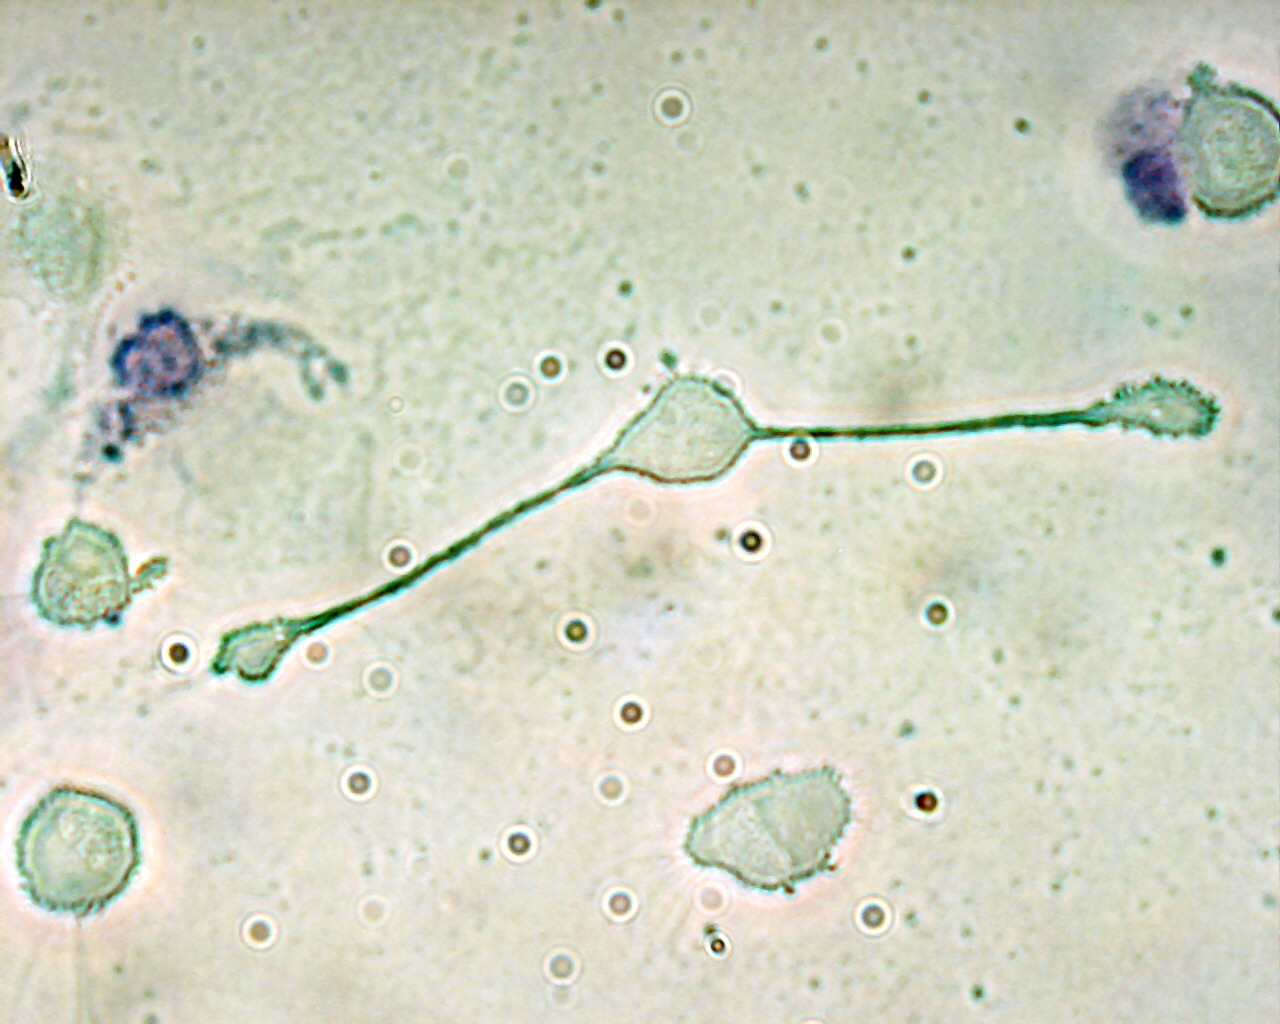
\includegraphics[width= 0.45 \textwidth]{img1.jpg} 
	\end{figure}
\end{frame}

\subsection{Dáta}
\begin{frame}{\textbf{Dáta}}
	\begin{itemize}
	\item Pri segmentácii sme primárne pracovali s 2D výsekom dát o veľkosti $80\times80$ pixlov.
	\item Ukážky výsekov pôvodných dát s ktorými sme pracovali:
	\end{itemize}
	\begin{figure}
	\centering
	  \subfloat[cropT2]{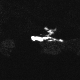
\includegraphics[width= 0.2 \textwidth]{cropT2.png}}
	  \qquad
      \subfloat[cropT7]{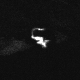
\includegraphics[width= 0.2 \linewidth]{cropT7.png}}
      	  \qquad
      \subfloat[cropT27]{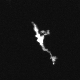
\includegraphics[width= 0.2 \linewidth]{cropT27.png}}
      	  \qquad
      \subfloat[cropT45]{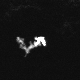
\includegraphics[width= 0.2 \linewidth]{cropT45.png}}
	\end{figure}
\end{frame}

\section{Prahovacie metódy}  

\begin{frame}{\textbf{Prahovacie metódy}}
	\begin{itemize}
	\item Prahovacie metódy slúžia na rozdelenie pôvodných dát do dvoch rôznych tried:
		\begin{itemize}
			\item \textbf{objekt},
			\item \textbf{pozadie}.
		\end{itemize}
	\vspace{2mm}
	\item Skúmali sme 2 rôzne typy prahovacích metód:
	\begin{itemize}
			\item \textbf{globálne prahovanie},
			\item \textbf{lokálne adaptívne prahovanie}.
		\end{itemize}
	\vspace{2mm}
	\item Výsledky prahovania použijeme pri výpočte segmentačnej metódy.
	\end{itemize}
\end{frame}

\subsection{Globálne prahovanie}
%\begin{frame}{\textbf{Globálne prahovanie}}{Otsuho prahovacia metóda}
%	\begin{itemize}
%	\item Pri výpočte prahu $q$
%	\item Otsuho prahovanie hľadá prah $q$, taký aby výsledné rozdelenie tried bolo čo najlepšie oddelené
%	\item \textbf{CO TU TREBA POVEDAT?}
%	\end{itemize}
%\end{frame}

%\begin{frame}{\textbf{Globálne prahovanie}}{Prahovanie pomocou maximálnej entropie}
%	\begin{itemize}
%	\item \textbf{Entropia} je štatistická miera, ktorá kvantifikuje priemerné množstvo informácií obsiahnutých v "správe" obsahujúce stochasticky generované dáta. Definovaná ako $$H(I)= -\sum^K_{i=0} p(g)log_b(p(g)),$$ kde $g$ je intenzita a $p(g)$ je pravdepodobnosť tejto intenzity v normalizovanom histograme.
%	\item 
%	\end{itemize}
%\end{frame}

\begin{frame}{\textbf{Globálne prahovanie}}
	\begin{itemize}
	\item Automatické prahovacie metódy.
		\vspace{2mm}

	\item Pre celé obrazové dáta hľadá jeden optimálny prah $q$.
		\vspace{2mm}

	\item Použité metódy: 
			\begin{itemize}
			\item Otsuho prahovanie,
			\item prahovanie pomocou maximálnej entropie.
			\end{itemize}
	\vspace{2mm}
	\item Nevyžadujú žiadne vstupy od používateľa.
	\end{itemize}
\end{frame}

\begin{frame}{\textbf{Globálne prahovanie}}{Výsledky}
	\begin{figure}
	\centering
	  \subfloat[cropT7]{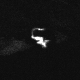
\includegraphics[width= 0.27 \textwidth]{cropT7.png}}
	  \qquad
      \subfloat[ Otsuho metóda \centering $prah = 108$]{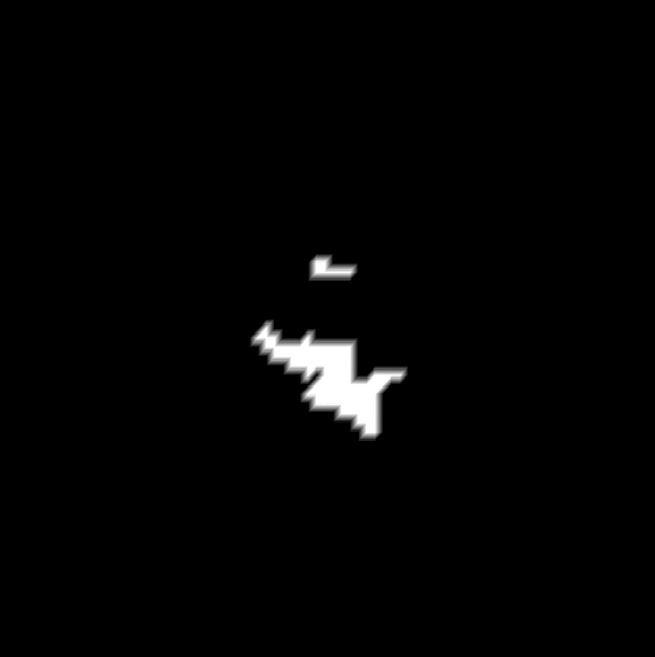
\includegraphics[width= 0.27 \linewidth]{cropT7_otsu.png}}
      	  \qquad
      \subfloat[ Pomocou max. \centering entropie $prah = 80$]{
\includegraphics[width= 0.27 \linewidth]{cropT7_kapur.png}}
	\end{figure}
\end{frame}

\begin{frame} {\textbf{Globálne prahovanie}}{Výsledky}
\begin{figure}
	\centering
	  \subfloat[cropT45]{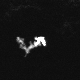
\includegraphics[width= 0.27 \textwidth]{cropT45.png}}
	    \qquad
      \subfloat[ Otsuho metóda \centering $prah = 105$]{
\includegraphics[width= 0.27 \linewidth]{cropT45_otsu.png}}
      \qquad
      \subfloat[ Pomocou max. \centering entropie $prah = 73$]{
\includegraphics[width= 0.27 \linewidth]{cropT45_kapur.png}}
	\end{figure}
\end{frame}

\subsection{Lokálne adaptívne prahovanie}
%\begin{frame}{\textbf{Lokálne adaptívne prahovanie}}{Niblackova metóda}
%	\begin{itemize}
%	\item
%	\end{itemize}
%\end{frame}

%\begin{frame}{\textbf{Lokálne adaptívne prahovanie}}{Sauvolova metóda}
%	\begin{itemize}
%	\item
%	\end{itemize}
%\end{frame}


%\begin{frame}{\textbf{Lokálne adaptívne prahovanie}}{Bernsenova metóda}
%	\begin{itemize}
%	\item
%	\end{itemize}
%\end{frame}

%\begin{frame}{\textbf{Lokálne adaptívne prahovanie}}{Hybridné metódy}
%	\begin{itemize}
%	\item
%	\end{itemize}
%\end{frame}

\begin{frame}{\textbf{Lokálne adaptívne prahovanie}}
\begin{itemize}
	\item Semi-automatické prahovacie metódy.
		\vspace{2mm}

	\item Pre každý pixel nachádzajúci sa na obrazových dátach vyhodnotí optimálny prah $q$.
		\vspace{2mm}
	\item Použité metódy: 
			\begin{itemize}
			\item Niblackova metóda,
			\item Bernsenova metóda,
			\item Sauvolova metóda,
			\item Hybridná Bernsen-Niblackova metóda,
			\item Hybridná Bernsen-Sauvolova metóda.
			\end{itemize}
	\vspace{2mm}
	\item Na vstup od používateľa ide veľkosť masky $m$ a v niektorých prípadoch aj veľkosť časového kroku $\sigma$.
	\end{itemize}
\end{frame}

\begin{frame}{\textbf{Lokálne adaptívne prahovanie}}{Výsledky}
		\begin{figure}
	\centering
	  \subfloat[cropT7]{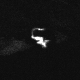
\includegraphics[width= 0.21 \textwidth]{cropT7.png}}
	  \qquad
      \subfloat[{\tiny Niblackova metóda \centering $m = 3, \sigma = 50.0$}]{
\includegraphics[width= 0.21 \linewidth]{cropT7_niblack.png}}
      \qquad
      \subfloat[{\tiny Bernsenova metóda \centering $m = 2$}]{
\includegraphics[width= 0.21 \linewidth]{cropT7_bernsen.png}}
      \qquad
      \subfloat[{\tiny Sauvolova metóda \centering $m = 3, \sigma = 50.0$}]{
\includegraphics[width= 0.21 \linewidth]{cropT7_sauvola.png}}
       \qquad
      \subfloat[{\fontsize{5.5}{4}\selectfont Bernsen-Niblackova m. \centering $m = 3, \sigma = 50.0$}]{
\includegraphics[width= 0.21 \linewidth]{cropT7_hybrid_nb.png}}
      \qquad
      \subfloat[{\fontsize{5.5}{4}\selectfont Bernsen-Sauvolova m. \centering $m = 3, \sigma = 50.0$}]{
\includegraphics[width= 0.21 \linewidth]{cropT7_hybrid_sb.png}}
	\end{figure}
\end{frame}

\begin{frame}{\textbf{Lokálne adaptívne prahovanie}}{Výsledky}
		\begin{figure}
	\centering
	  \subfloat[{\tiny cropT45}]{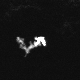
\includegraphics[width= 0.21 \textwidth]{cropT45.png}}
	  \qquad
      \subfloat[{\tiny Niblackova metóda \centering $m = 3, \sigma = 50.0$}]{
\includegraphics[width= 0.21 \linewidth]{cropT45_niblack.png}}
      \qquad
      \subfloat[{\tiny Bernsenova metóda  $m = 2$}]{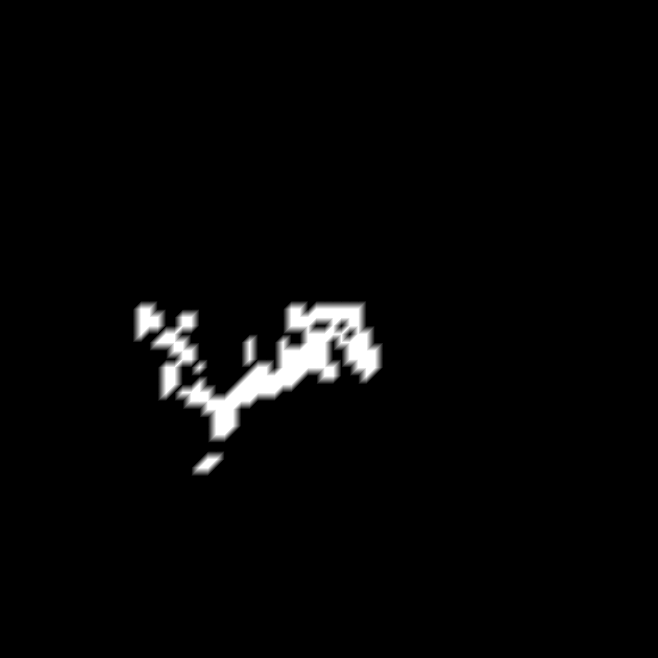
\includegraphics[width= 0.21 \linewidth]{cropT45_bernsen.png}}
      \qquad
      \subfloat[{\tiny Sauvolova metóda \centering $m = 3, \sigma = 50.0$}]{
\includegraphics[width= 0.21 \linewidth]{cropT45_sauvola.png}}
       \qquad
      \subfloat[{\fontsize{5.5}{4}\selectfont Bernsen-Niblackova m. \centering $m = 3, \sigma = 50.0$}]{
\includegraphics[width= 0.21 \linewidth]{cropT45_hybrid_nb.png}}
      \qquad
      \subfloat[{\fontsize{5.5}{4}\selectfont Bernsen-Sauvolova m. \centering $m = 3, \sigma = 50.0$}]{
\includegraphics[width= 0.21 \linewidth]{cropT45_hybrid_sb.png}}
	\end{figure}
\end{frame}

\section{Segmentačná metóda}

\begin{frame}{\textbf{Segmentačná metóda (SUBSURF)}}
	\begin{itemize}
	\item Parciálna diferenciálna rovnica má tvar
	$$
u_t = \sqrt{\epsilon^2 + |\nabla u|^2}\nabla.\left(g \frac{\nabla u}{\sqrt{\epsilon^2 + |\nabla u|^2}}\right),
$$
ktorá sa dá upraviť do advekčno-difúzneho tvaru ako 

	$$
u_t-\nabla g\cdot \nabla u=g \sqrt{\epsilon^2 + |\nabla u|^2}\nabla.\left( \frac{\nabla u}{\sqrt{\epsilon^2 + |\nabla u|^2}}\right),
$$

kde $g$ predstavuje funkcia

	 $$g(s) = \frac{1}{1+ks^2}, k > 0,$$
kde $s = |\nabla G_{\sigma} * I^0|$ predstavuje normu gradientu predvyhladených dát.
	\end{itemize}
\end{frame}

\begin{frame}{\textbf{Segmentačná metóda (SUBSURF)}}
	\begin{itemize}
	\item Použili sme dve modifikácie funkcie $g$:
	\begin{itemize} 
	\item $g1(u_o , u_t) = \frac{1}{1 + k|\nabla \frac{u_o + u_t}{2}|^2},$
	\item $g2(u_o , u_t) = \frac{0.2}{1 + k|\nabla u_o|^2} + \frac{0.8}{1 + k|\nabla u_t|^2},$
	\end{itemize}
	kde $u_o$ predstavujú pôvodné dáta a $u_t$ sú vyprahované dáta.
	\vspace{2mm}
	\item Počiatočná podmienka:
	\begin{itemize}
	\item výsledok z prahovania,
	\item znamienkova funkcia vzdialenosti.
	\end{itemize}
	\vspace{2mm}	
	\item V ukážkových príkladoch bol použitý difúzny koeficient $g2$ spolu so znamienkovou funkciou vzdialenosti. 
	\end{itemize}
\end{frame}

\section{Výsledky}

\begin{frame}{\textbf{Výsledky segmentačnej metódy}}{použité dáta \textit{cropT7.pgm}}
\begin{itemize}
\item {\small Vstupné parametre metódy: $t = 15, \sigma = 0.5, \tau = 1.0, k = 500, z = -1.5$.}
\end{itemize}
	\begin{figure}
	\centering
      \subfloat[\centering Pomocou max. entropie]{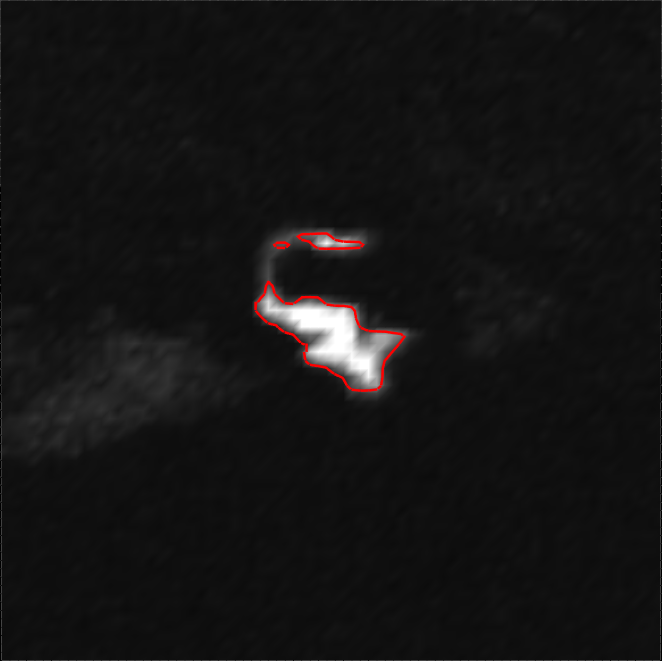
\includegraphics[width= 0.35 \linewidth]{cropT7_kapur_sdf.png}}
      \qquad
    \subfloat[\centering Hybridná Bernsen-Niblackova metóda]{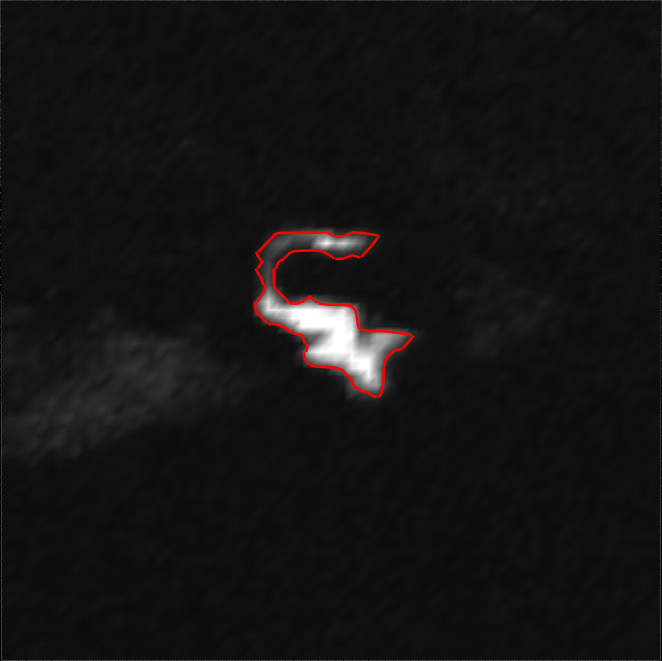
\includegraphics[width= 0.35 \linewidth]{cropT7_hybrid_nb_sdf.png}}
	\end{figure}
\end{frame}

\begin{frame}{\textbf{Výsledky segmentačnej metódy}}{použité dáta \textit{cropT45.pgm}}
	\begin{figure}
	\centering
      \subfloat[ Pomocou max. \centering entropie]{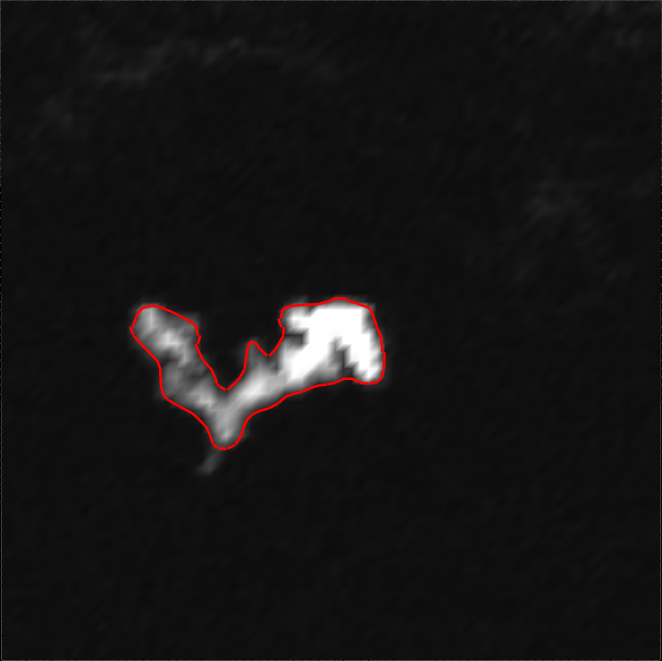
\includegraphics[width= 0.35 \linewidth]{cropT45_kapur_sdf.png}}
      \qquad
    \subfloat[\centering Hybridná Bernsen-Niblackova metóda]{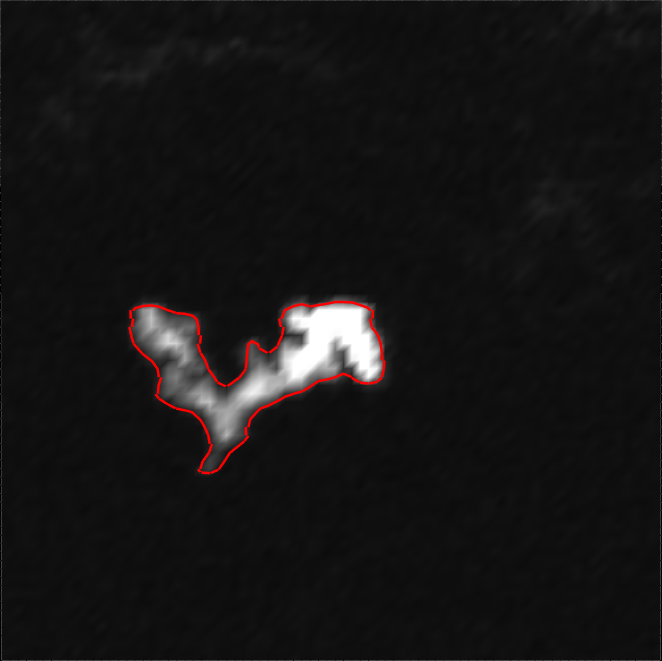
\includegraphics[width= 0.35 \linewidth]{cropT45_hybrid_nb_sdf.png}}
	\end{figure}
\end{frame}

\begin{frame}{\textbf{Výsledky segmentačnej metódy}}
		\begin{figure}
	\centering
	  \subfloat[Výrez $350\times150 pixlov$ z pôvodných dát]{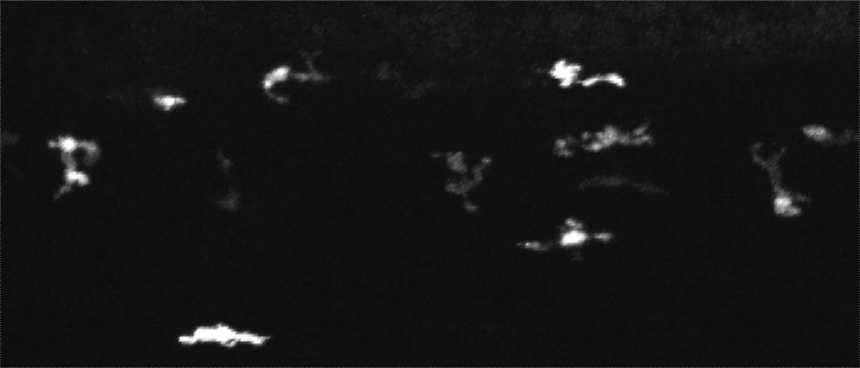
\includegraphics[width= 1 \textwidth]{vysekoD.png}}
	\end{figure}
\end{frame}

\begin{frame}{\textbf{Výsledky segmentačnej metódy}}{{}}
		\begin{figure}
	\centering
      \subfloat[\centering {\tiny Prahovanie pomocou maximálnej entropie}]{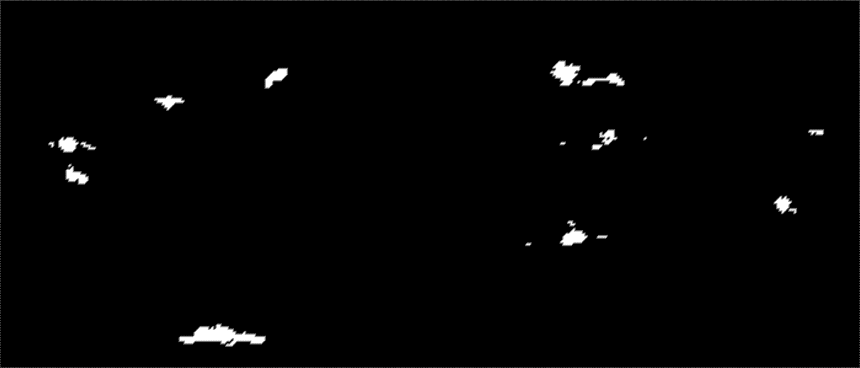
\includegraphics[width= 0.5 \linewidth]{vysek_kapur.png}}
	  \qquad
      \subfloat[\centering  {\tiny Hybridná Bernsen-Niblackova metóda $m = 5, \sigma = 50.0$}]{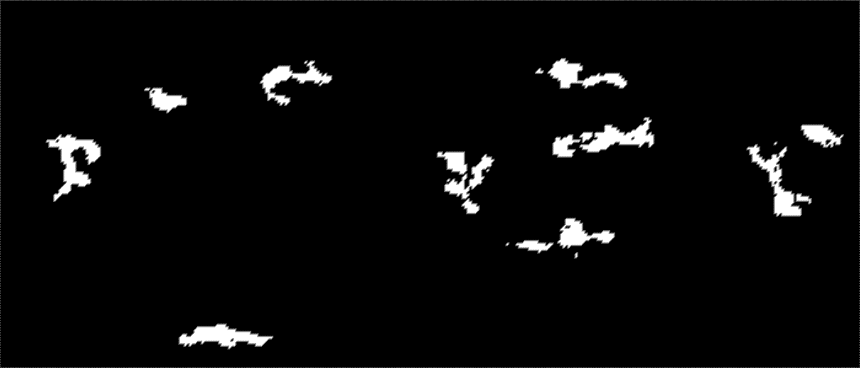
\includegraphics[width= 0.5 \linewidth]{vysek_hybrid_nb.png}}
	\end{figure}
\end{frame}

\begin{frame}{\textbf{Výsledky segmentačnej metódy}}
\begin{itemize}
\item {\small Vstupné parametre metódy: $t = 10, \sigma = 0.5, \tau = 1.0, k = 500, z = -1.5$.}
\end{itemize}
		\begin{figure}
	\centering
      \subfloat[\centering {\tiny Výsledok segmentačnej metódy pri použití globálneho prahovania}]{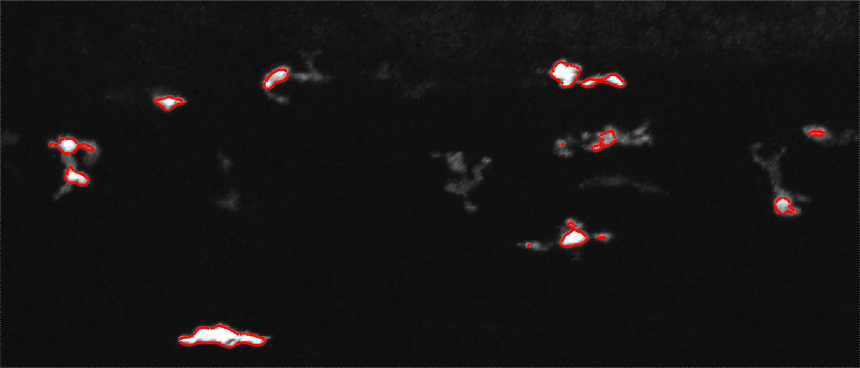
\includegraphics[width= 0.47 \linewidth]{vysek_kapur_res.png}}
	  \qquad
      \subfloat[\centering  {\tiny Výsledok segmentačnej metódy pri použití lokálneho adaptívneho prahovania}]{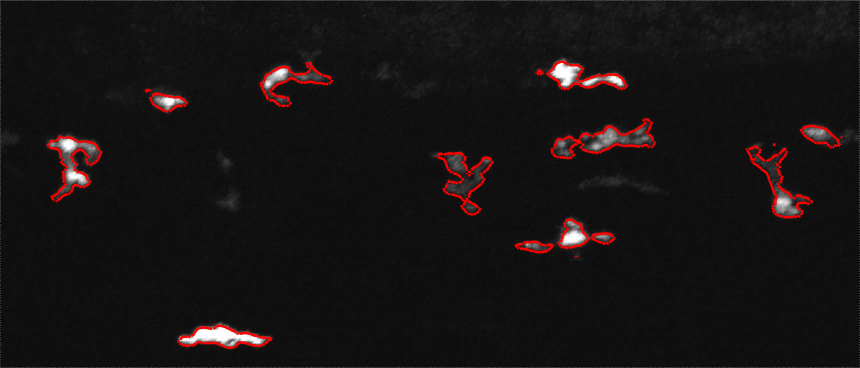
\includegraphics[width= 0.47 \linewidth]{vysek_hybrid_nb_res.png}}
	\end{figure}
\end{frame}


%\begin{frame}
%\begin{columns}
%\column{0.5\textwidth}
%\begin{figure}
%	\centering
%      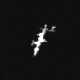
\includegraphics[width= 1 \textwidth]{img4.jpg} 
%      \caption{Original data}
%	\end{figure}
%\column{0.5\textwidth}
%\begin{figure}
%	\centering
%      
\includegraphics[width= 1 \textwidth]{img5.jpg} 
%       \caption{Otsu's thresholding method}
%	\end{figure}
%\end{columns}
%\end{frame}

%\subsection{Maximum entropy thresholding}
%\begin{frame}{\textbf{Kapur's thresholding method}}{Maximum entropy thresholding}
%	\begin{itemize}
%	\item \textbf{Entropy} is a statistical measure of randomness that can be used to characterize the texture of the input image.
%	\item Entropy is defined as  $H(I)= -\sum_{u,v} p(g)log_b(p(g))$, where $g$ is probability of each intensity and $p(g)$ is probability distribution.
%	\item Because the maximized entropy is needed, it will be defined with following formulas
	
%	\begin{equation*}
%		H_0(q) =  -\frac{1}{P_0(q}S_0(q)+log(P_0(q)),
%	\end{equation*}
%	\begin{equation*}
%		H_1(q) =  -\frac{1}{1-P_0(q)}S_1(q)+log(1-P_0(q)),
%	\end{equation*}
%where $P_0$ is cumulative probability and $S_0$, $S_1$ are summation terms. 
%	\end{itemize}
%\end{frame}

%\begin{frame}{\textbf{Kapur's thresholding method}}{Maximum entropy thresholding}
%	\begin{itemize}
%	\item Cumulative probabilities:
	
%	$P_0(q) = \begin{cases} p(0) & \text{for } q = 0 \\
%                           P_0(q-1) + p(q)         & \text{for } 0 < q < L      %
%       \end{cases}$
%          \vspace{2mm}
%    \item Summation terms:   
    
%    $S_0(q) = \begin{cases} p(0).log(p(0))) & \text{for } q = 0 \\
%                            S_0(q-1) + p(q)log(p(q))         & \text{for } 0 < q < L      %
%        \end{cases}$
%        \vspace{1mm}
%	$S_1(q) = \begin{cases} 0 & \text{for } q = L-1 \\
%                            S_0(q+1) + p(q+1)log(p(q+1))         & \text{for } 0 \leq q < L -1      %
%        \end{cases}$       	
	
%	\end{itemize}
%\end{frame}

%\begin{frame}
%\begin{columns}
%\column{0.5\textwidth}
%\begin{figure}
%	\centering
%      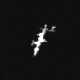
\includegraphics[width= 1 \textwidth]{img4.jpg} 
%      \caption{Original data}
%	\end{figure}
%\column{0.5\textwidth}
%\begin{figure}
%	\centering
%     
\includegraphics[width= 1 \textwidth]{img6.jpg} 
%       \caption{Kapur's thresholding method}
%	\end{figure}
%\end{columns}
%\end{frame}

%\subsection{Comparison}
%\begin{frame} {\textbf{Comparison}}
%\begin{columns}
%\column{0.3\textwidth}
%\begin{figure}
%	\centering
%      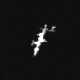
\includegraphics[width= 1\textwidth]{img4.jpg} 
%      \caption{Original
%       data}
%	\end{figure}
%	\vspace{1mm}
%\column{0.3\textwidth}
%\begin{figure}
%	\centering
%      
\includegraphics[width= 1 \textwidth]{img5.jpg} 
%      \caption{Otsu's thresholding method}
%	\end{figure}
%\column{0.3\textwidth}
%\begin{figure}
%	\centering
%      
\includegraphics[width= 1 \textwidth]{img6.jpg} 
%       \caption{Kapur's thresholding method}
%	\end{figure}
%\end{columns}
%\end{frame}

%\begin{frame} {\textbf{Comparison with Wolfram Mathematica }}
%\begin{columns}
%\column{0.5\textwidth}
%\centering
%\textbf{Otsu's thresholding method}
%\begin{minipage}[c][0.4\textheight][c]{\linewidth}
%  \centering
%  
\includegraphics[width=0.55\linewidth]{img5.jpg}
%\end{minipage}
%\begin{minipage}[c][0.4\textheight][c]{\linewidth}
%  \centering
%  
\includegraphics[width=0.55\linewidth]{img7.jpg}
%\end{minipage}
%\begin{figure}
%      
\includegraphics[width=0.5 \textwidth]{img5.jpg} 
%	 \hfill
%      
\includegraphics[width= 0.5 \textwidth]{img7.jpg} 
%	\end{figure}
%\column{0.5\textwidth}
%\centering
%\textbf{Kapur's thresholding method}
%\begin{minipage}[c][0.4\textheight][c]{\linewidth}
%  \centering
%  
\includegraphics[width=0.55\linewidth]{img6.jpg}
%\end{minipage}
%\begin{minipage}[c][0.4\textheight][c]{\linewidth}
%  \centering
%  
\includegraphics[width=0.55\linewidth]{img8.jpg}
%\end{minipage}
%\begin{figure}
%	\centering
%      
\includegraphics[width= 1 \textwidth]{img6.jpg} 
%	\end{figure}
%	\begin{figure}
%	\centering
%      
\includegraphics[width= 1 \textwidth]{img8.jpg} 
%	\end{figure}
%\end{columns}
%\end{frame}

\section{Software}

\begin{frame}{\textbf{Software}}
	\begin{itemize}
	\item Program je implementovaný v objektovo-orientovanom jazyku C++. 
	
	\vspace{2mm}
	\item Na vytvorenie užívateľského prostredia (GUI) boli použité Qt knižnice.
	
	\vspace{2mm}
	\item Visualization Toolkit knižnice (VTK) boli použité na zobrazovanie a manipuláciu s dátami.
	\end{itemize}
\end{frame}

\begin{frame}{\textbf{Software}}
\begin{figure}
	\centering
       \subfloat[Ukážka grafického rozhrania so zobrazenými 2D dátami.]{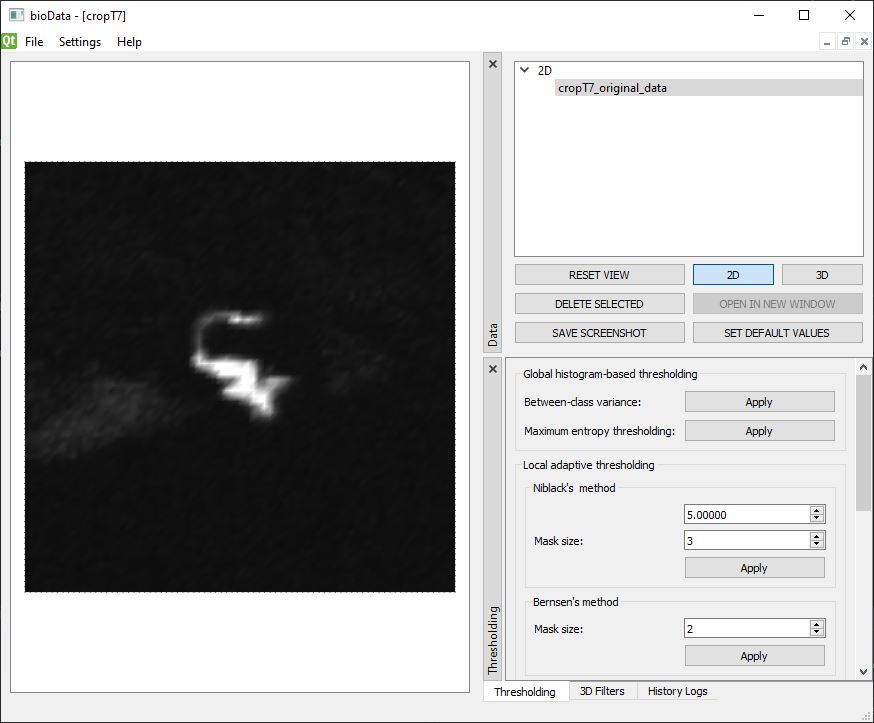
\includegraphics[width= 0.6 \linewidth]{ui.jpg}}
       %\caption{Kapur's thresholding method}
	\end{figure}
\end{frame}

\begin{frame}{\textbf{Software}}
\begin{figure}
	\centering
      \subfloat[Ukážka grafického rozhrania so zobrazenými 3D dátami - výsledkom zo segmentačnej metódy.]{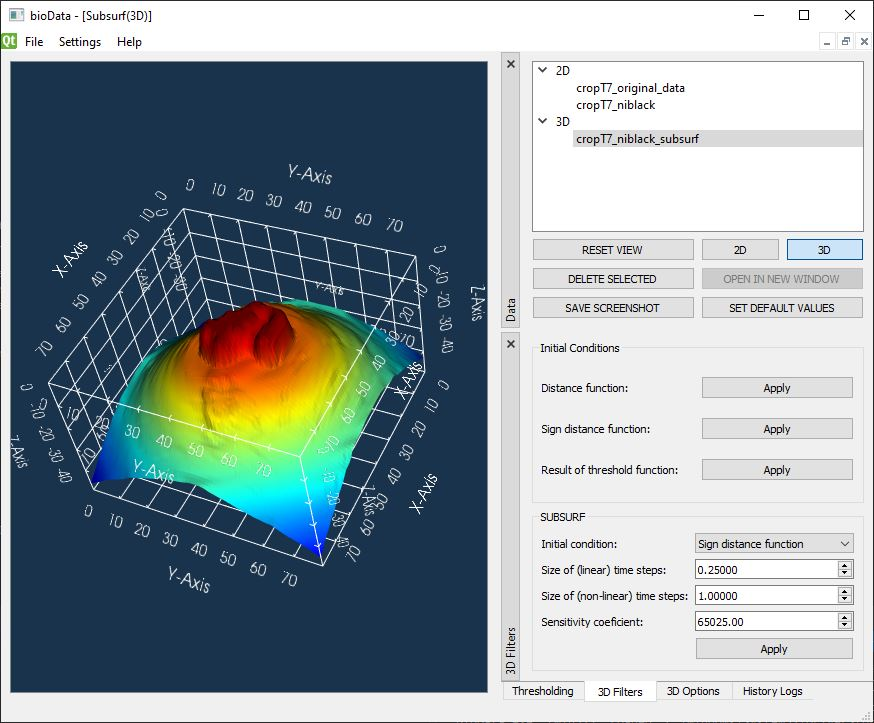
\includegraphics[width= 0.6 \linewidth]{subsurf.jpg}}
       %\caption{Kapur's thresholding method}
	\end{figure}
\end{frame}

\section*{Ďakujem za pozornosť}
\begin{frame}
  \begin{center}
  	\vspace{0.7cm}
		\textbf{\LARGE Ďakujem za pozornosť!}
  \end{center}
\end{frame}

\section*{Porovnanie metód}
\begin{frame}{Modifikácia difúzneho koeficientu}
\begin{figure}
	\centering
      \subfloat[Pri použití funkcie $g1$]{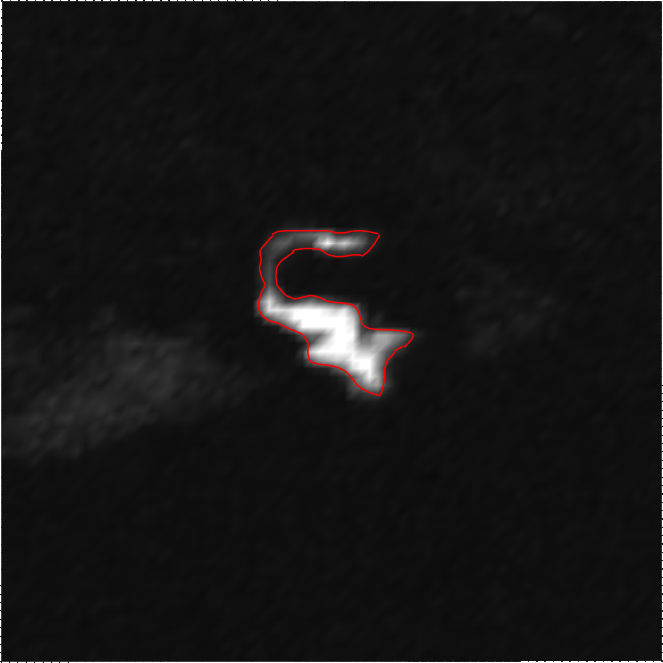
\includegraphics[width= 0.45 \linewidth]{grad1.png}}
       \qquad
       \subfloat[Pri použití funkcie $g2$]{\includegraphics[width= 0.45 \linewidth]{grad2.png}}
       %\caption{Kapur's thresholding method}
	\end{figure}
\end{frame}

\begin{frame}{Typ počiatočnej podmienky}
\begin{columns}
\begin{column}{0.5\textwidth}
\centering
  Znamienková funkcia vzdialenosti
  \begin{figure}
	\centering
      \subfloat[{\tiny počiatočná podmienka}]{\includegraphics[width= 0.45 \textwidth]{1.png}}
       %\caption{Kapur's thresholding method}
        \qquad
       \subfloat[{\tiny výsledok segmentácie}]{\includegraphics[width= 0.5 \linewidth]{grad2.png}}
	\end{figure}
\end{column}
\begin{column}{0.5\textwidth}  %%<--- here
\centering
  Výsledok z prahovania
  \begin{figure}
	\centering
      \subfloat[{\tiny počiatočná podmienka}]{\includegraphics[width= 0.45 \textwidth]{2.png}}
       %\caption{Kapur's thresholding method}
        \qquad
       \subfloat[{\tiny výsledok segmentácie}]{\includegraphics[width= 0.5 \linewidth]{3.png}}
	\end{figure}
\end{column}
\end{columns}
\end{frame}

\section*{Do budúcna}
\begin{frame}{Do budúcna}
\begin{itemize}
\item Sprehľadniť grafické rozhranie.
	\vspace{2mm}
\item Vyhodnotiť kvalitu výsledkov inak, ako len vizuálne napríklad pomocou Hausdorffovej vzdialenoti.
	\vspace{2mm}
\item Možnosť využitia dávkového spracovania.
	\vspace{2mm}
\item Paralelizácia pri práci s väčšími dátami.
	\vspace{2mm}
\item Kompilácia pre novšiu verziu VTK knižníc.
\end{itemize}
\end{frame}

\end{document}
